%***********************************************************************
% Lab Report Template
% R. W. Melton
% May 19, 2019
% August 24, 2020
%***********************************************************************
%Modify the following macros to set document property values
%used for cover sheet (title page) and page header
\newcommand{\CourseNumber}{CMPE-250}
\newcommand{\CourseName}{Assembly and Embedded Programming}
\newcommand{\SemesterName}{Fall 2020}
\newcommand{\SemesterCode}{20201}
\newcommand{\LabExNum}{2}
\newcommand{\LabExTitle}{Basic Arithmetic Operations}
\newcommand{\StudentName}{Andrei Tumbar}
\newcommand{\DateSubmit}{09-01-20}
\newcommand{\LabSection}{1}
\newcommand{\LabInstructor}{Melton}
\newcommand{\TAa}{Cameron Hudson}
\newcommand{\TAb}{Chris Augsburger}
\newcommand{\TAc}{Anthony Bacchetta}
\newcommand{\LectureSection}{1}
\newcommand{\LectureInstructor}{Melton}
%End macros for document property values
%***********************************************************************
\title{Lab Ex. \LabExNum\ Report}
\author{\StudentName}
\date{\DateSubmit}
\makeatletter %make \title, \author, and \date availabile with \@
\newcommand{\FontSize}{12}
\newcommand{\FontUnit}{pt}
\newcommand{\HeadSize}{\dimexpr \FontSize\FontUnit + 2pt \relax}
\documentclass[\FontSize\FontUnit,letterpaper,oneside]{article}
\usepackage[twoside=false,margin=1in]{geometry}
\usepackage[utf8]{inputenc}
\usepackage[USenglish]{babel}
\usepackage{graphicx}
\usepackage[normalem]{ulem}
\usepackage{newtxtext, newtxmath}
%If newtx package had to be installed in multiuser environment
%regular user may have to run updmap command to avoid following error
%FATAL:  ``PK font ts1-qtmr could not be created.'' in miktex-makepk
%Alternatively, uncomment the following line
%\pdfmapfile{=pdftex35.map
\usepackage{booktabs}
\usepackage{enumitem}
\usepackage{nameref}
\usepackage[pdfborder={0 0 0},plainpages=false,pdfpagelabels]{hyperref}
\def\code#1{\texttt{#1}}
%If hyperref generates errors on first build, rebuild.            
\hypersetup{pdfauthor={\@author},
            pdftitle={\@title},
            pdfsubject={\CourseNumber\ \SemesterCode},
            %pdfkeywords={},
            %pdfproducer={Latex with hyperref, or other system},
            %pdfcreator={pdflatex, or other tool}
            urlcolor=none}
\setlength{\topsep}{\z@}
\setlength{\partopsep}{\z@}
\setlength{\itemsep}{\z@}
\setlength{\parindent}{\z@}
\setlength{\parskip}{\FontSize\FontUnit plus 2pt minus 1pt}
\setlength{\baselineskip}{\dimexpr \FontSize\FontUnit + 2pt \relax}
\renewcommand \baselinestretch{1}
\makeatletter
  \renewcommand \section{
    \@startsection{section}{1}{\z@}
      %Before 2 lines, accounting for normal \parskip
      {\dimexpr \FontSize\FontUnit * 2 - \parskip \relax plus 0pt minus 0pt}
      %After 1 line, accounting for normal \parskip
      {0.1pt plus 2pt minus 1pt} %nonzero amount to get normal \parskip
      {\normalfont\normalsize\bfseries}} 
  \renewcommand \subsection{
    \@startsection{paragraph}{2}{\z@}
      %Before 1 lines, accounting for normal \parskip
      {0.1pt plus 2pt minus 1pt}
      %After 0.5 em on same line as heading
      {-0.5em} 
      {\normalfont\normalsize\bfseries}} 
  \renewcommand \subsubsection{
    \@startsection{paragraph}{3}{\z@}
      %Before 1 line, accounting for normal \parskip
      {0.1pt plus 2pt minus 1pt}
      %After 0.5 em on same line as heading
      {-0.5em} 
      {\normalfont\normalsize\uline}} 
  \renewcommand \paragraph{
      \@startsection{paragraph}{4}{\z@}
      %Before 1 line, accounting for normal \parskip
      {0.1pt plus 2pt minus 1pt}
      %After 0.5 em on same line as heading
      {-0.5em} 
      {\normalfont\normalsize}} 
\makeatother
\pagenumbering{arabic}
\headheight=\HeadSize
\usepackage{fancyhdr}
\renewcommand{\headrulewidth}{0pt}
\renewcommand{\footrulewidth}{0pt}
\makeatletter %make \title, \author, and \date availabile with \@
\pagestyle{fancy}
\fancyhead{} %clear all header fields
\fancyhead[L]{\small \CourseNumber\ \SemesterCode \@author:  \@title}
\fancyhead[R]{\small Page \thepage\ of \pageref*{LastPage}}
\fancyfoot{} %clear all footer fields
\fancypagestyle{plain}{
  \renewcommand{\headrulewidth}{0pt}
  \renewcommand{\footrulewidth}{0pt}
  \fancyhf{} %clear header and footer fields
  \fancyfoot[C]{\small \CourseNumber\ \SemesterCode\ \@author:  \@title:  
    Page \thepage\ of \pageref*{LastPage}}
}
%May require second build to get correct page numbers.            
\begin{document}
\raggedbottom
\widowpenalties 1 10000
\lefthyphenmin=4
\righthyphenmin=4
\setlist{nolistsep}
%***********************************************************************
%Title page is automatically generated from macros at top of file
\pagenumbering{roman}
\begin{titlepage}
  %No space before paragraph at top of page
  %\vspace{\dimexpr-2\parsep-2\parskip\relax}
  %1.5 in before center (list) at top of page
  \vspace*{\dimexpr 1.5in - \topsep - \partopsep - \topskip - \parskip \relax}
  \begin{center}
    \textbf{\large\CourseNumber\ \CourseName\linebreak
      \linebreak
      Laboratory Exercise \LabExNum\linebreak
      \linebreak
      \LabExTitle}
  \end{center}
  \vspace*{\dimexpr 1.5in - \topsep - \partopsep - \topskip \relax}
  \par By submitting this report, I attest that its contents are wholly 
    my individual writing about this exercise and that they reflect 
    the submitted code.  I further acknowledge that permitted 
    collaboration for this exercise consists only of discussions of 
    concepts with course staff and fellow students.  Other than code 
    provided by the instructor for this exercise, all code was 
    developed by me.
  \null
  \vspace*{4\parskip}
  \hspace*{3.25in}\begin{tabular}[t]
    {@{\hskip0pt}r    %Specification
     @{\hskip1em}l    %Value
     @{\hskip0pt}}
    \toprule[1pt]
    \multicolumn{2}{l}{\StudentName}\\
    \multicolumn{2}{l}{\DateSubmit}\\
    \\
    Lab Section:&\LabSection\\
    Instructor:&\LabInstructor\\
    TA:&\TAa\\
    &\TAb\\
    &\TAc\\
    \\
    Lecture Section:&\LectureSection\\
    Lecture Instructor:&\LectureInstructor
  \end{tabular}
\end{titlepage}
\pagenumbering{arabic}
\thispagestyle{plain}
%***********************************************************************
%Report body begins here
\section*{Abstract}

\par In this laboratory exercise, basic arithmetic operations were performed
to evaluate students' profficiency with simple assembly instructions. A given
arithmetic expression was provided. Intermediate results were calculated 
before writing the assembly instructions so that the code could be debugged
after writing. The assembly instructions included moving constants into registers
and performing arithmetic operations such as addition, subtraction, multiplication,
and division. Assembly was written for ARM Cortex-M0+ processors.

\section*{Procedure}

This exercise was built around calculating the value of the following arithmetic
expression:

\begin{equation*}
18 + ([-11] \div 2) + 13 + (5 \cdot 9) - 42 + 3
\end{equation*}

One of the requirements is that all constants that can be seen in the expression, must
be loaded into registers before they are used. Immediate values used in bitshifting
operations do not need to be loaded beforehand.

By continuously loading \code{R0} with the intermediate result of each step, more registers
are left free for other operations. To compute the result from the equation above, use \code{R1}
to first store $-11$ and then divide by $2$ (perform with a right-arithmetic shift by one bit). 
Follow-up by storing $18$ into \code{R0} and adding \code{R0} and \code{R1}. This result should
be stored back into \code{R0}.

\code{R0} should now have the result from computing $18 + ([-11] \div 2)$. The rest of the expression
can be completed using the same method. The multiplication $5 \cdot 9$ can be performed by calculated
$5 \cdot 8 + 5$. Multiplication by a power $2$ can also be expressed by the following:

\begin{equation*}
\alpha \cdot 2^\beta = \alpha << \beta 
\end{equation*}

This calculation can be performed using the $R1$ register because the previous result is no
loonger needed. The rest of the expression is simply performed using \code{ADDS} and \code{SUBS}
operations.

\section*{Results}

The expression should yield the result of $31$. This is because $\frac{-11}{2}$
is an integer division and should therefore yield $-6$ instead of $-5.5$. $31$ 
in hex is \code{0x1F}. After the assembly instructions were written, the program
was run with the debugger to verify the results. A screen capture was taken after
the final instruction was performed.

\pagebreak

\begin{figure}[h!]
	\centering
	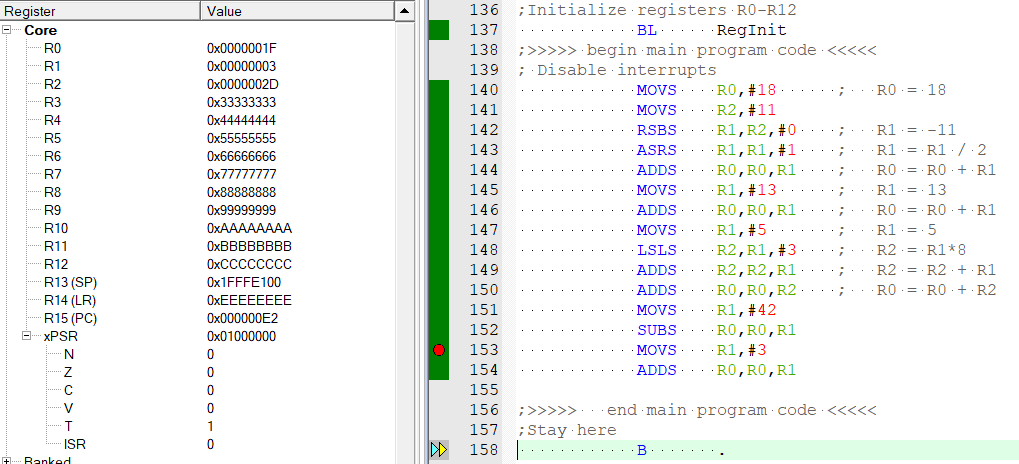
\includegraphics[width=\textwidth]{capture}
	\caption{Debugger results after program execution.}
	\label{fig:capture}
\end{figure}

Figure 1 shows the values of every register. Line 137 initialy fills every register with
\code{RN=0xNNNNNNNN}. General purpose registers \code{R3} and above were never used and
therefore still contain the values they were initalized with. \code{R0} holds the result
of the expression in question, \code{0x1F} or $31$ in base 10 which matches the prediction.

\section*{Conclusion}
%\par The conclusion section provides the reader with insights that came from 
%  completing the lab exercise.  It describes the lessons learned in the 
%  exercise and analyzes the results.  It also notes and explains any 
%  deviations from the assigned procedure.  It concludes by describing 
%  general concepts applied to achieve the results and by making 
%  statements that extend beyond the scope of the exercise to the general 
%  case, (e.g., where the concepts or results could be applied outside of 
%  the lab exercise).

This laboratory exercise was important because it taught students basic assembly instructions
and program flow as well as how to effectively use the debugger. By calculating intermediate
values before the program is written and including pseudo-code along with the assembly instructions,
the program was very easy to debug. These basic assembly skills can be applied to more complex 
programs because they provide the more basic operations and computations.


\label{LastPage}
\end{document}
